\chapter{Heartbleed}
\label{chapter:Heartbleed}

\section{Présentation}
\paragraph{}
Heartbleed\up{\cite{article:Heartbleed2}}, présente depuis mars 2012, a été révélée en avril 2014 par l'équipe de sécurité de Google et des ingénieurs de Codenomicon (société finlandaise). C'est une vulnérabilité logicielle due à une erreur de programmation dans la librairie openSSL.

Contrairement aux attaques précédentes qui ciblent assez clairement les informations à extraire, Heartbleed ne permet pas de choisir ce que l'on veut récupérer. Un attaquant utilisant cette attaque peut lire la mémoire d'un serveur et peut récupérer aussi bien des clés privées que des choses sans importance.

\section{Comment ça marche}
\paragraph{}
Le problème vient de l'extension heartbeat qui permet, sans renégociation, de demander au serveur si la connexion est toujours active. Le fonctionnement du protocole est le suivant :
\begin{itemize}
  \item Le navigateur envoie une requête au serveur en lui demandant, si la connexion est toujours active, de lui renvoyer "ack" qui fait 3 lettres.
  \item Le serveur reçoit la demande et répond en lui envoyant :
  	\begin{verbatim}
		ack
	\end{verbatim}
\end{itemize}

\paragraph{}
Il faut savoir que lorsqu'un serveur reçoit une requête, il l'enregistre dans ses logs. Un attaquant sachant cela peut modifier légèrement la requête pour récupérer de l'information.
\begin{itemize}
  \item Le navigateur de l'attaquant envoie une requête au serveur en lui demandant, si la connexion est toujours active, de lui renvoyer "ack" qui fait 250 lettres.
  \item Le serveur reçoit la demande et répond en lui envoyant :
	\begin{verbatim}
		ack
		[Admin:ID1]
		[Session:d3cb1acdbbadbef32efsdecf98ce3b2c1]
		[Demande:status]
		[Status:OK]
		[Clé privée de transation:5c4a5e5c3b1ce3ef2fa3c3b39e498fcd]
		[Hash du mot de passe:b1ce3eabcedfa9456f2fa3c3b398c9e4d]
		[Demandé:3 lettres:"ACK"]
		[Envoyé:"ACK"]
		[Marie:ID84]
	\end{verbatim}
\end{itemize}

\paragraph{}
Le serveur va en fait prendre en compte la longueur demandé et non la taille du mot demandée. Ainsi, bien que le navigateur demande au serveur de lui renvoyer "ack", le serveur va déborder dans sa mémoire et renvoyer les logs d'autres requêtes.\\

\begin{figure}[h]
\label{fig:Heartbleed}
\centering
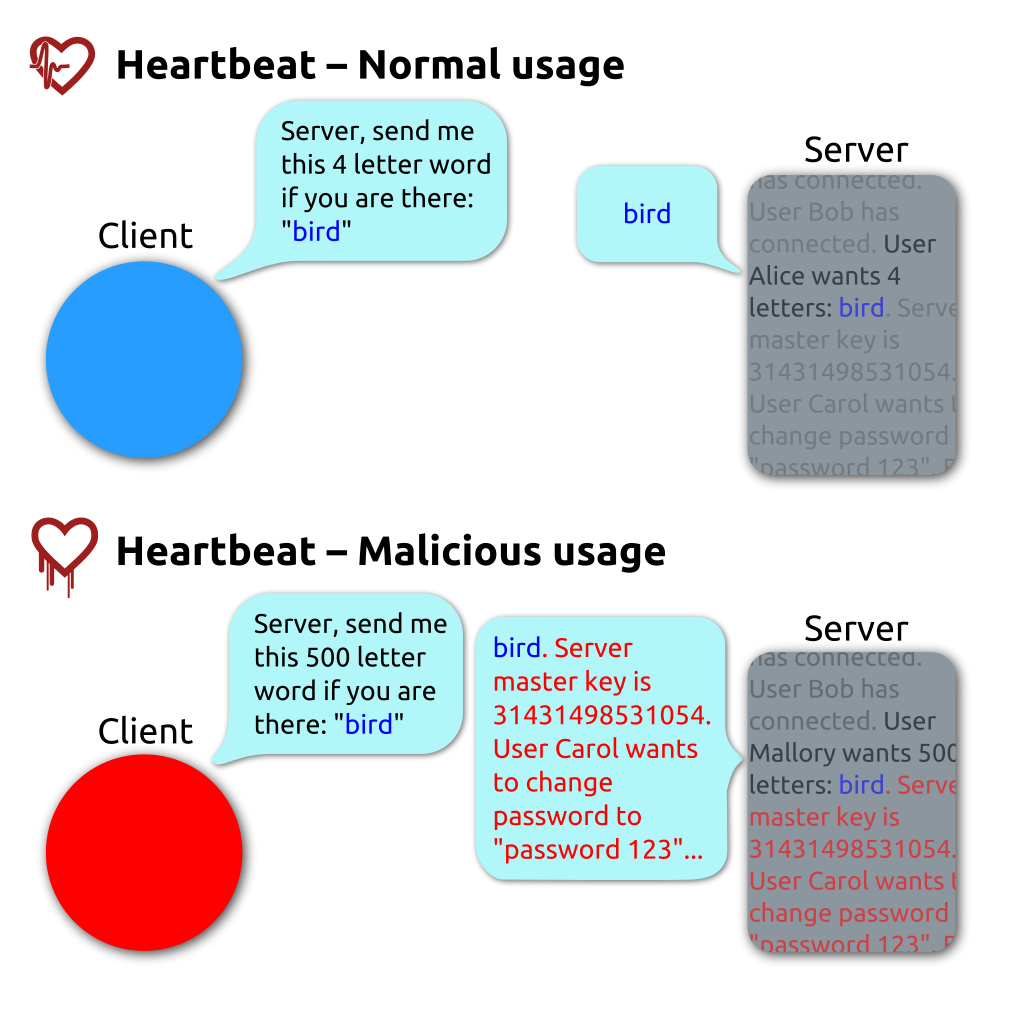
\includegraphics[scale=0.2]{Heartbleed}
\caption{Principe de Heartbleed\up{\cite{article:Heartbleed}}}
\end{figure}

Ci-dessous est présentée la structure d'un message Heartbeat\up{\cite{article:ZDNet}}.
\begin{verbatim}
struct {
HeartbeatMessageType type;
uint16 payload_length;
opaque payload[HeartbeatMessage.payload_length];
opaque padding[padding_length];
} HeartbeatMessage;
\end{verbatim}

On peut remarquer que la longueur du message envoyé par le client est codée sur 16 bits. Un attaquant peut donc, théoriquement, récolter $2^{16} (= 64Ko)$ caractères.

\section{Contre-mesures}
\paragraph{}
Le code à l'origine de cette faille à d'ores et déjà été modifié. Il suffit donc d'utiliser la dernière version de TLS pour être à l'abri. Si cela n'est pas possible, il faut alors désactiver l'extension heartbeat.
